%% Toffoli gate
%
% The Toffoli gate -- a NOT on the third qubit controlled by the first two, the
% gate the modular arithmetic of Shor's algorithm is built from -- and its
% decomposition into gates of one qubit and controlled NOTs: H, T and its
% adjoint, and six CNOTs, in thirteen steps.
%
% Time runs down: a qubit is a site and a step of the circuit a layer, so a
% gate on one qubit is a tensor in a slot, and a controlled NOT a dot and a
% circled plus in one layer, joined along it. Where a CNOT acts on the first
% and the third qubit, the second qubit's wire crosses its line (+). The
% layers of gates on one qubit are apart, with nothing along them.
%
% Thirteen steps would be half a page tall at the notation's distances; the
% circuit is drawn compact instead -- both stacks at 0.7 of the notation's
% distances and sizes, the decomposition's layers closer still -- by factors,
% not lengths.
\documentclass[border=4pt]{standalone}
\usepackage{amsmath,amssymb}
\usepackage{tikz-tensors}
\input{notation}
\begin{document}
\begin{tikzpicture}
  \tnstack[scale=0.7]{G}{3}{x}
  \tnlayer{G}{x}{2*ctrl/, targ/}
  \tnconnect{G}
  \tnopen[labels={$a$, $b$, $c$}]{up}{G}
  \tnopen{down}{G}
  \tneq
  \tnstack[scale=0.7, rise=0.6]{D}{3}{h1, x1, t1, x2, t2, x3, t3, x4, t4, h2, x5, t5, x6}
  \tnlayer{D}{h1}{2*|, gate/$H$}
  \tnlayer{D}{x1}{|, ctrl/, targ/}
  \tnlayer{D}{t1}{2*|, gate/$T^\dagger$}
  \tnlayer{D}{x2}{ctrl/, +, targ/}
  \tnlayer{D}{t2}{2*|, gate/$T$}
  \tnlayer{D}{x3}{|, ctrl/, targ/}
  \tnlayer{D}{t3}{2*|, gate/$T^\dagger$}
  \tnlayer{D}{x4}{ctrl/, +, targ/}
  \tnlayer{D}{t4}{|, 2*gate/$T$}
  \tnlayer{D}{h2}{2*|, gate/$H$}
  \tnlayer{D}{x5}{ctrl/, targ/, |}
  \tnlayer{D}{t5}{gate/$T$, gate/$T^\dagger$, |}
  \tnlayer{D}{x6}{ctrl/, targ/, |}
  \tnconnect[apart={h1, t1, t2, t3, t4, h2, t5}]{D}
  \tnopen[labels={$a$, $b$, $c$}]{up}{D}
  \tnopen{down}{D}
\end{tikzpicture}
\end{document}
